\subsubsection{Descripci\'on} 
\newpage
\subsubsection{C\'odigo} 
\lstinputlisting{r_code/redundancy.R}
\newpage
\subsubsection{Ejemplo} 
\subsubsection{Comparativa/Versiones} 
\begin{figure}[h]
    \centering
    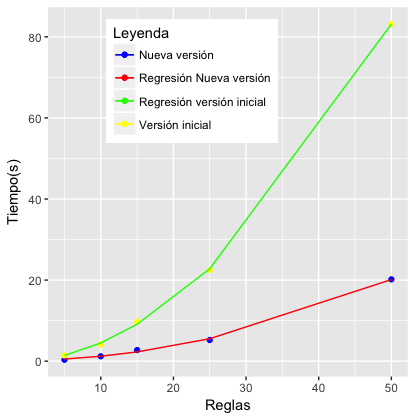
\includegraphics[scale=0.75]{Redundancy}
    \caption{Pruebas remove.redundancy}
    \label{fig:redundancy}
\end{figure} 

En la figura \ref{fig:redundancy} podemos ver una grafica comparativa entre dos versiones distintas de esta funcion. La primera de ellas es la version de la que disponia el director de este TFG en el momento en que se empezo a desarrollar el mismo. La segunda es una version mejorada (como se puede ver mas arriba en el extracto de codigo), que se realizo como parte de este trabajo.